%%====================%%
%%  Part III Project  %%
%%====================%%

\documentclass[aps,prd,reprint,preprintnumbers,showpacs,floatfix,nofootinbib,superscript address]{revtex4-2}
\usepackage[utf8]{inputenc}
\usepackage{parskip}
\usepackage{amssymb}
\usepackage{stix}
\usepackage{hhline}
\usepackage{amsmath}
\usepackage{mathtools}
\usepackage[dvipsnames]{xcolor}
\usepackage{xspace}
\usepackage{multirow,tabularx}
\usepackage{siunitx}
\usepackage{multirow}
\usepackage{graphicx}
\usepackage{xstring}
\usepackage{etoolbox}
\usepackage{notoccite}
\usepackage{natbib}
\usepackage{mathrsfs}
\usepackage{lineno}
\usepackage{tensor}
\usepackage{accents}
\usepackage{tikz}
\usepackage{listings}
\allowdisplaybreaks
\parskip 1mm
\parindent 2mm

%%===========================%%
%%  Part III Project Macros  %%
%%===========================%%

%	The Planck mass
\newrobustcmd{\Planck}{%
	{M_{\text{Pl}}}%
}

%	The Riemannian covariant derivative
\newrobustcmd{\rD}[1]{%
	\tensor{\mathring{\nabla}}{#1}%
}

%	The Riemann-Cartan covariant derivative
\newrobustcmd{\rcD}[1]{%
	\tensor{\nabla}{#1}%
}

%	The Riemann tensor
\newrobustcmd{\rR}[1]{%
	\tensor{\mathring{R}}{#1}%
}

%	The Riemann-Cartan tensor
\newrobustcmd{\rcR}[1]{%
	\tensor{R}{#1}%
}

%	Irreducible parts of the torsion
\newrobustcmd{\T}[2][placeholder]{%
	\IfEqCase{#1}{%
	{placeholder}{\tensor{T}{#2}}%
	{1}{\tensor[^{(1)}]{T}{#2}}%
	{2}{\tensor[^{(2)}]{T}{#2}}%
	{3}{\tensor[^{(3)}]{T}{#2}}%
	}%
	[\packageError{cosmicclass}{Symbol #1 is not an irreducible part!}{}]%
}

%	Irreducible parts of the multiplier
\newrobustcmd{\TLambda}[2][placeholder]{%
	\IfEqCase{#1}{%
	{placeholder}{\tensor{\lambda}{#2}}%
	{1}{\tensor[^{(1)}]{\lambda}{#2}}%
	{2}{\tensor[^{(2)}]{\lambda}{#2}}%
	{3}{\tensor[^{(3)}]{\lambda}{#2}}%
	}%
	[\packageError{cosmicclass}{Symbol #1 is not an irreducible part!}{}]%
}
 %some personal macros

\usepackage{hyperref}
\hypersetup{%
     colorlinks = true,%
     linkcolor = Blue,%
     citecolor = Blue,%
     filecolor = Blue,%
     urlcolor = Blue% 
     }%
\usepackage[capitalize]{cleveref} %always load this last in preamble

\newcommand{\signature}[2][8em]{%
  \begin{tabular}[t]{ p{#1} p{#1} }
    \strut\raggedleft
    \raisebox{-.5ex}[0pt][0pt]{\bfseries #2} & \\
    \cline{2-2}
    & \centering\scriptsize\itshape (signature)
  \end{tabular}
}

\usepackage[style=nejm, 
citestyle=numeric-comp,
sorting=none]{biblatex}
\addbibresource{Bibliography.bib}


\nocite{*}

\begin{document}
\title{Constraints on inflation from scale-invariant gravity}

\author{Prabhoda CS}
\affiliation{Department of Physics, Cavendish Laboratory, University of Cambridge}

\begin{abstract}

\textbf{TO BE WRITTEN}
\textit{Italics sections to be edited... and more}
\end{abstract}

\maketitle


\section{The need for Inflation}\label{The need for Inflation}

\indent The simplest model of the Big Bang theory naturally follows from General Relativity applied to a general isotropic and homogeneous universe (Friedmann Equations) combined with Hubble's observations (Hubble's Law). This theory describes a universe with a constant expansion rate. It is a highly successful theory, able to offer a comprehensive explanation for a lot of experimental observations such as the CMB, the abundance of light elements, large scale structure and mainly, Hubble's Law.

However, there are several problems with this simple model. In the following section, we will present two arguments against the conventional Big Bang theory.

\subsection{Horizon Problem}
In this section, we will show that given the standard assumed expansion rate in the big bang model, we cannot satisfactorily explain the near-perfect uniformity of the CMB. This is because, given the rate of expansion, there is no way for distant regions of the CMB to have once been causally connected.
Given the Friedmann Equations and defining the Hubble constant $H = \frac{\dot{a}}{a}$,
\begin{equation} \label{1}
    \dot{\rho} = -3(\rho + p)H
\end{equation}
\begin{equation} \label{2}
    \Ddot{a} = -\frac{4\pi G}{3} (\rho + 3p)a
\end{equation}
\begin{equation}    \label{3}
    H^2 + \frac{k}{a^2} = \frac{8 \pi G}{3} \rho
\end{equation}

From the continuity equation \ref{1}, we have:
\begin{equation} \label{4}
    \frac{\mathrm{d}  \ln(\rho)}{\mathrm{d} \ln(a)} = -3(1+w)
\end{equation}

Where, $w = \frac{p}{\rho}$. We can solve this equation to get $\rho \propto a^{-3(1+w)}$. In combination with Friedmann equation \ref{3} for a flat universe $k = 0$, we get the scale factor $a$ as a function of time $a(t)$.

\begin{equation}    \label{5}
    a(t) = \begin{cases}
        t^{2/3(1+w)} & w \neq -1 \\
        e^{Ht} & w = -1
    \end{cases}
\end{equation}

Now, we can define the comoving horizon ($\tau$) as the causal horizon or the maximum distance a light ray can travel between times 0 and $t$.

\begin{equation}    \label{6}
    \tau \equiv \int_{0}^{t} \frac{\mathrm{d} t'}{a(t')} = \int_{0}^{a} \frac{\mathrm{d}a}{H a^2} = \int_{0}^{a} \mathrm{d} \ln(a) \frac{1}{aH}
\end{equation}

For a conventional Big Bang model, therefore, the causal horizon $\tau$ for a universe with $w \geq 0$ increases with time. In plain words, this means that the fraction of the universe with each other increases with time.
\begin{equation}
    \tau \propto a^{1/2(1+3w)} \implies \tau = \begin{cases}
        a & \text{Radiation Dominated} \\
        a^{1/2} & \text{Matter Dominated}
    \end{cases}
\end{equation}

The comoving horizon increasing with time implies that comoving scales (comoving scale is not the same as the physical scale) entering the cosmic horizon now were not in causal contact during the CMB decoupling! However, the anisotropy of the CMB is about one part in $10^{-5}$, posing a problem to the conventional big bang model to explain how these distant regions of the CMB managed to regulate their temperatures to such an accurate degree.

\subsection{Flatness Problem}
We know that despite the presence of mass and energy in our universe, the large scale structure of out spacetime is approximately Euclidean (flat). To see whether this is a stable equilibrium, we return to Friedmann equation \ref{3} and defining $\rho_{\text{crit}} = 3H^2(a)$ and $\Omega(a) = \frac{\rho(a)}{\rho_{\text{crit}}}$, we get
\begin{equation}
    1 - \Omega(a) = \frac{-k}{(aH)^2}
\end{equation}
Differentiating this equation and using the Friedmann equations, we get,
\begin{equation}
    \frac{\mathrm{d}\Omega}{\mathrm{d} \ln a} = (1+3w)\Omega(\Omega-1)
\end{equation}
Looking at this, we can see that $\Omega = 1  \implies \rho = \rho_{crit}$ is an unstable equilibrium and slight perturbations can make the universe not flat i.e., $k \neq 0$. This means that in the standard big bang model, matter density has to be extremely fine tuned to fit the requirement $\rho = \rho_{crit}$, which seems unlikely.

The theory of inflation attempts to resolve the need for extreme fine tuning of the initial conditions of the universe by positing a period of exponential expansion. The next section shows how this theory solves the two problems stated above.

\section{Inflation}\label{Inflation}

Looking at both the problems highlighted in the previous section, we see that the comoving Hubble radius ($(aH)^{-1}$) plays an important role
\begin{equation}    \label{10}
    \tau = \int_{0}^{a} \mathrm{d} \ln (a) \frac{1}{aH}
\end{equation}
\begin{equation} \label{11}
    1 - \Omega (a) = \frac{-k}{(aH)^2}
\end{equation}
If the comoving Hubble radius was decreasing, this means that large scales entering the present universe were inside the horizon before inflation. By equation \ref{11}, it also means that $\rho = \rho_{crit}$ is a stable equilibrium as the solution $\Omega = 1$ is an attractor during inflation.

A decreasing comoving horizon directly implies a period of accelerated expansion as seen by taking it's derivative
\begin{equation}
    \frac{\mathrm{d}}{\mathrm{d}t} \frac{1}{aH} <  0 \implies \frac{-\Ddot{a}}{(aH)^2} < 0 \implies \ddot{a} > 0
\end{equation}
Given that $\ddot{a} > 0$ and Friedmann equation \ref{2}, we see that $\frac{\rho}{3} < p \implies w < - \frac{1}{3}$. This is a violation of the strong energy condition.

So far, we have described the physical implications of inflation and it's effects. In the following section, we shall describe the physical conditions under which such an exponential expansion can arise. 

\subsection{Non-Canonical Scalar Field Inflation}
The simplest models of inflation involve a scalar field $\phi$ (The Inflaton Field) that acts as the perfect fluid with $w < -\frac{1}{3}$ such that upon coupling with gravity through the Einstein-Hilbert action, it can provide the repulsive force in the Friedmann equations for the accelerated expansion.

In this section, we shall work with a general non-canonical scalar field and derive the equations of motion and relevant parameters for such a scalar field. This will provide us with the necessary groundwork for what is to come later in our model.

\begin{equation}\label{12}
    S = \int \mathrm{d}^4 x \sqrt{-g} \left[ g^{\mu \nu} \frac{K(\phi)}{2} \partial_{\mu}\phi \partial_{\nu} \phi  - V(\phi) \right]\
\end{equation}

Since during the inflationary period, we assume a de Sitter space (minus the perturbations), the FLRW metric is given by $g_{\mu \nu}= \text{diag}[1,-a^2(t),-a^2(t),-a^2(t)]$ making $\sqrt{-g} = a^3(t)$. We also assume that the scalar field is homogeneous and therefore only varies with time, allowing us to drop the gradient term. The action then becomes: 

\begin{equation} \label{13}
    S = \int \text{dt}\text{d}^3\text{x} \; \text{a}^3(t) \left[ \frac{K(\varphi)}{2}\dot{\varphi}^2 - V(\varphi) \right]
\end{equation}

We vary the action and upon integrating by parts we get,

\begin{equation}
    \delta S = - \int \text{dt}\,\text{d}^3\textbf{x} \; \left[ a^3 K \ddot{\varphi} + a^3K_{,\varphi} \frac{\dot{\varphi}^2}{2}  +  3\dot{a} a^2 K \dot{\varphi} + a^3V_{,\varphi}  \right]\delta \varphi
\end{equation}

Setting this variation to zero, we get the equation of motion for a non-canonical scalar field.

\begin{equation} \label{16}
    K \ddot{\varphi} + \dot{\varphi} \left(\frac{K_{,\varphi} \dot{\varphi}}{2} + 3H K \right) + V_{,\varphi}   = 0
\end{equation}

We see this aligns with the canonical scalar field when we set $K = 1$, getting  $ \ddot{\varphi} +  3H \dot{\varphi}  + V_{,\varphi}   = 0$. While this equation is nice, it turns out to be more useful in cosmology to record how the inflaton field changes with respect to the e-folding time ($N = \int H \text{d}t$). For this, let us take an aside and given the action \ref{12}, derive the energy-momentum tensor.

\begin{equation}
    T_{\mu\nu} = \frac{2}{\sqrt{-g}} \frac{\delta S}{\delta  g^{\mu \nu}} = \frac{\partial \mathcal{L}}{\partial (\partial^\mu \phi)} \partial_\nu \phi - g_{\mu\nu} \mathcal{L}
\end{equation}

Using this, and simplifying the final expression we get, the energy density and the pressure of the fluid are as follows: 

\begin{align}
    \rho &= \frac{K(\varphi)}{2} \dot{\varphi}^2 + V(\varphi) \nonumber \\
    p &= \frac{K(\varphi)}{2} \dot{\varphi}^2 - V(\varphi)
\end{align}

Using the third Friedmann equation \ref{3}, we get:

\begin{equation}    \label{Friedmann Eqn 2}
    3 M_p^2H^2 = \frac{K(\varphi)}{2} \dot{\varphi}^2 + V(\varphi)
\end{equation}

Upon differentiating this expression with respect to time and using \ref{16}, we get:

\begin{equation}
    2 M_p^2 \dot{H} = -  K \dot{\varphi}^2
\end{equation}

Now that we have all the relevant parameters as functions of the field, we can look at equation \ref{16} and replace the time derivative there with the derivative with respect to the e-folding time N. Using $\text{d}N = H \text{d}t$, we get our final answer of the field evolution as a differential equation with respect to N.

\begin{widetext}
\begin{subequations}
\begin{align}\label{21}
    K\frac{\text{d}^2\varphi}{\text{d}N^2} +3 K \frac{\text{d}\varphi}{\text{d}N}  - \frac{K^2}{2M_p^2} \left(\frac{\text{d}\varphi}{\text{d}N} \right)^3  +  \frac{K_{,\varphi}}{2}  \left(\frac{\text{d}\varphi}{\text{d}N} \right)^2 +  \left( 3 M_p^2 - \frac{K}{2} \left(\frac{\text{d}\varphi}{\text{d}N} \right)^2 \right) \frac{\text{d}\ln \text{V}(\varphi)}{\text{d} \varphi} = 0    
\end{align}
\end{subequations}
\end{widetext}

\subsection{Slow Roll Inflation}
The acceleration equation for universe dominated by the inflaton field with the energy density $\rho_{\phi}$ and pressure $p_{\phi}$ is given by Friedmann equation \ref{2},
\begin{equation}
    \frac{\ddot{a}}{a} = -\frac{4\pi G}{3} (\rho +3p) = -\frac{8\pi G}{3} ({\dot{\phi}}^2 - V(\phi)) 
\end{equation}
We see that if we can get $\ddot{a} > 0$ by requiring $\dot{\phi}^2 << |V(\phi)|$. This period is called slow roll because when this condition is satisfied, it corresponds to the scalar field slowly rolling down its potential hill. The accelerated expansion will also only be satisfied for a long period if we require $|\ddot{\phi}| << 3H\dot{\phi} \sim |V,_{\phi}|$. 

We can rewrite these two slow-roll conditions with the two slow-roll parameters $\epsilon$ and $\eta$ and requiring that $\epsilon_V << 1$ and $\eta_V << 1$ during the slow roll. 
\begin{equation}
    \epsilon_V = \frac{1}{2}  \left( \frac{V,_{\phi}}{V} \right)^2 \,\,\,\,\,\,\,\,\ \eta_V = \left| \frac{V,_{\phi\phi}}{V} \right|
\end{equation}

We can also write down the Hubble Slow Roll parameters (HSR), which are easily computable for our case of a non-canonical action:

\begin{align}
    \epsilon_H &= -  \left( \frac{\dot{H}}{H^2} \right) = \frac{K(\phi)}{2 M_p^2} \left( \frac{\text{d}\phi}{\text{d}N} \right)^2  \nonumber \\
    \eta_H &= \epsilon_H - \frac{1}{2 \epsilon_H} \left( \frac{\text{d}\epsilon_H}{\text{d}N} \right)
\end{align}

Inflation ends exactly when the HSR hits one, that is, $\epsilon_H = 1$.

So far, these arguments only provide restrictions on the potential of the scalar field $\phi$, but make no attempt to motivate the form of the potential or the action principle for the field from first principles. Thus, we see that the theory of inflation refers to a whole host of theories that aim to explain the mechanism behind the period of exponential expansion that occurred when the universe was around $\geq 10^{-34}s$ old.

\textit{One of the ways to arrive at the action principle of the inflaton field is to take a leaf out of the playbook of many successful QFTs and to hypothesize a gauge condition. This is the approach that shall be taken in this project and explained more in the next section.}


\section{Scale Invariant Gravity} \label{Section 3}
Having laid the groundwork, we now come to the primary study of this project. This is based on the paper \cite{barker2024poincaregaugetheoryconformal} mainly and will follow up on the idea and analyze the theory with the inclusion of gravity. This immediately makes the theory much richer producing various inflationary scenarios such as hilltop, plateau (Starobinsky-like), and even power law/ exponential potentials.

The theory of General Relativity is one of mankind's most rigorous scientific theories, is self-consistent and so far, all tests of GR have been shown to be in agreement with the theory. However, we do not \textit{a priori} know that the theory of general relativity can be extended to arbitrary energy (/length) scales. It is widely accepted that at high enough energy scales, those comparable to the Planck scale, GR breaks down. 

An interesting possibility to consider is that GR as we know it, with the Einstein-Hilbert lagrangian being proportional to the Ricci Scalar, is a low-energy extrapolation of a more fundamental scale-invariant theory that describes physics at higher energies. Scale invariance in cosmology seems quite an attractive hypothesis given the nearly scale-invariant spectrum of primordial fluctuations as measured by Planck and WMAP. It shall be shown in the later part of the paper that the desired plateau form of the Starobinsky potential also arises from the inclusion of $R^2$ term in the Lagrangian. Given $[R^2] = 4$ in natural units, its coefficient is naturally dimensionless and therefore invariant under change of scale $g_{\mu\nu} \rightarrow \Omega^2 g_{\mu\nu}$, for $\Omega$ constant. Another approach to inflationary cosmology is to consider metric-affine theories. This is done through the inclusion of the Holst invariant, a quantity that is already scale-invariant, in the lagrangian. This has been explored in \cite{Salvio_2022} and \cite{pradisi2022equivalence}. The potential achieved in \cite{Salvio_2022} is identical to the one obtained through demanding scale invariance in \cite{barker2024poincaregaugetheoryconformal} and the translation between the variables in the two theories will be given in the Appendix. Finally, when considering the classical action of the Standard Model, dropping the Higgs mass terms, one finds that it too is scale-invariant and can be extended to be conformally invariant \cite{bars2014local}. 

All of these investigations may hint towards a fundamental principle out of which these arise as limits - \textit{the inflaton potential arising} due to the gauging of this scale invariance, i.e., conformal symmetry.

In the argument that follows, we derive the most general conformally invariant action with non-irrelevant couplings of the inflaton field and gravity. We do not consider terms proportional to the curvature squared, even though this is a perfectly legal and general extension of the model. It is easy to show that this results in a two-field inflation model. We find, however, that the proceeding model that we will derive is quite general and accounts for a lot of behaviors seen in the potentials derived through other means. Let us begin by exploring this possibility with a spin-0 scalar field that is minimally coupled to gravity.

\begin{equation} \label{25}
    S = \int \mathrm{d}^4 x \sqrt{-g} \frac{1}{2} \left[ \partial_\mu \varphi \partial^\mu \varphi - m^2   \varphi^2   \right] + \text{gravity}
\end{equation}

Under local rescalings, the metric and the scalar transforms as $g_{\mu\nu} \rightarrow e^{2\rho} g_{\mu\nu} $ and  $\varphi \rightarrow e^{-\rho}\varphi$ respectively. To ensure the kinetic terms retain their form, we introduce the Weyl vector $B_\mu$ which transforms as such $B_{\mu} \rightarrow B_\mu - \partial_\mu \rho$ under the gauge transformation (going back to the roots of the word) and define the covariant derivative $D_\mu = \partial_\mu - B_\mu$. To remove the explicit mass scale $m$ appearing in the Lagrangian \ref{25}, we add a compensator scalar field $\phi \rightarrow e^{-\rho}\phi$. For the gravity sector of the Lagrangian, let us see how the Christoffel symbol transforms under a local rescaling:

\begin{equation}
    \tilde{\Gamma}^{\alpha}_{\beta \gamma} = \Gamma^{\alpha}_{\beta \gamma} +(\delta^{\alpha}_{\beta} \partial_\gamma \rho + \delta^{\alpha}_{\gamma} \partial_{\beta} \rho - g_{\beta \gamma}g^{\alpha \tau}\partial_{\tau}\rho)
\end{equation}

Defining a new connection that is conformally covariant using $B_\mu$ and using that to define the new curvature scalar, we get the Weyl curvature scalar:

\begin{align}
    \mathcal{T}^{\alpha}_{\beta \gamma} &= \Gamma^{\alpha}_{\beta \gamma} + (\delta^{\alpha}_{\beta} B_{\gamma} + \delta^{\alpha}_{\gamma} B_{\beta} - g_{\beta \gamma}g^{\alpha \tau}B_{\tau}) \nonumber \\
    \tilde{R} &= R - 6 B_{\mu} B^{\mu} - 6 \nabla_\mu B^\mu
\end{align}

Putting all this together, we get the most general conformally invariant action, (assuming linearity in the curvature)

\begin{widetext}
\begin{subequations} \label{28a}
\begin{align}
    S =\int \text{d}^4\text{x} \; \sqrt{-g} &\; \left[ ( \beta \varphi^2 + \gamma \phi \varphi +\alpha \phi^2) R - 6( \beta \varphi^2 + \gamma \phi \varphi +\alpha \phi^2) (B_{\mu} B^{\mu} - \nabla_\mu B^\mu) \right. \nonumber \\
    &\quad \left. +\frac{\epsilon}{2} D_{\mu}\varphi D^{\mu}\varphi + \frac{\sigma}{2} D_{\mu}\varphi D^{\mu}\phi + \frac{\nu}{2} D_{\mu}\phi D^{\mu}\phi \right. \nonumber\left. - \frac{\mu^2}{2} \phi^2 \varphi^2 + \frac{\lambda}{2} \varphi^4 + \frac{\kappa}{2} \phi^4 - \frac{\xi}{16} H_{\mu\nu}H^{\mu\nu} \right] \,.\label{28a} 
\end{align}
\end{subequations}
\end{widetext}

A point to note here is the abundance of dimensionless parameters. We can remove any two of them by rescaling our fields, but we will leave it in this form until necessary. In the proceeding discussions, we shall set $\lambda = \kappa = 0$, this can be reinstated in the end, once the dynamics have been analyzed and the final inflaton potential is revealed.

In the equation above, we find that there are two scalar fields here. This makes analyzing the equations of motion harder. However, we have a redundant degree of freedom granted to us through the Weyl invariance we demanded the action possess. Looking at the units of $[\phi] = 2$, which is inverse length. Since the action is written down to be invariant under any choice of scale, we can choose a particular local length scale such that the field $\phi$ no longer appears dynamical, that is, rescale the metric and fields such that $\phi(\text{x}^\mu) = \phi_0$. The reparametrizations that allows us to do this are : $g_{\mu \nu} \rightarrow \frac{\phi_0}{\phi} g_{\mu \nu}$, $\varphi \rightarrow \frac{\phi}{\phi_0} \varphi$ and $B_{\mu} \rightarrow B_{\mu} - \partial_{\mu} ln(\phi)$. The resulting action in the Jordan Frame therefore reads:

\begin{equation}
    \begin{aligned}
        \mathcal{L} &= ( \beta \varphi^2 + \gamma \phi_0 \varphi +\alpha \phi^2_0) (R - 6B_{\mu} B^{\mu} - 6\nabla_\mu B^\mu) \\
        &+ \frac{\epsilon}{2} (\partial_\mu \varphi - (\varphi + \frac{\sigma}{\epsilon} \phi_0)B_\mu)(\partial^\mu \varphi - \varphi B^\mu)\\
        &- \frac{\mu^2}{2} \phi^2_0 \varphi^2 + \frac{\nu \phi_{0}^{2}}{2} B_\mu B^\mu - \frac{\xi}{16} H_{\mu\nu}H^{\mu\nu}
    \end{aligned}
\end{equation}


\textbf{CHANGE FROM HERE ONWARDS...}




We can see the graph of the potential in Fig \ref{Potential from Paper}.
\begin{figure}[h]
    \centering
    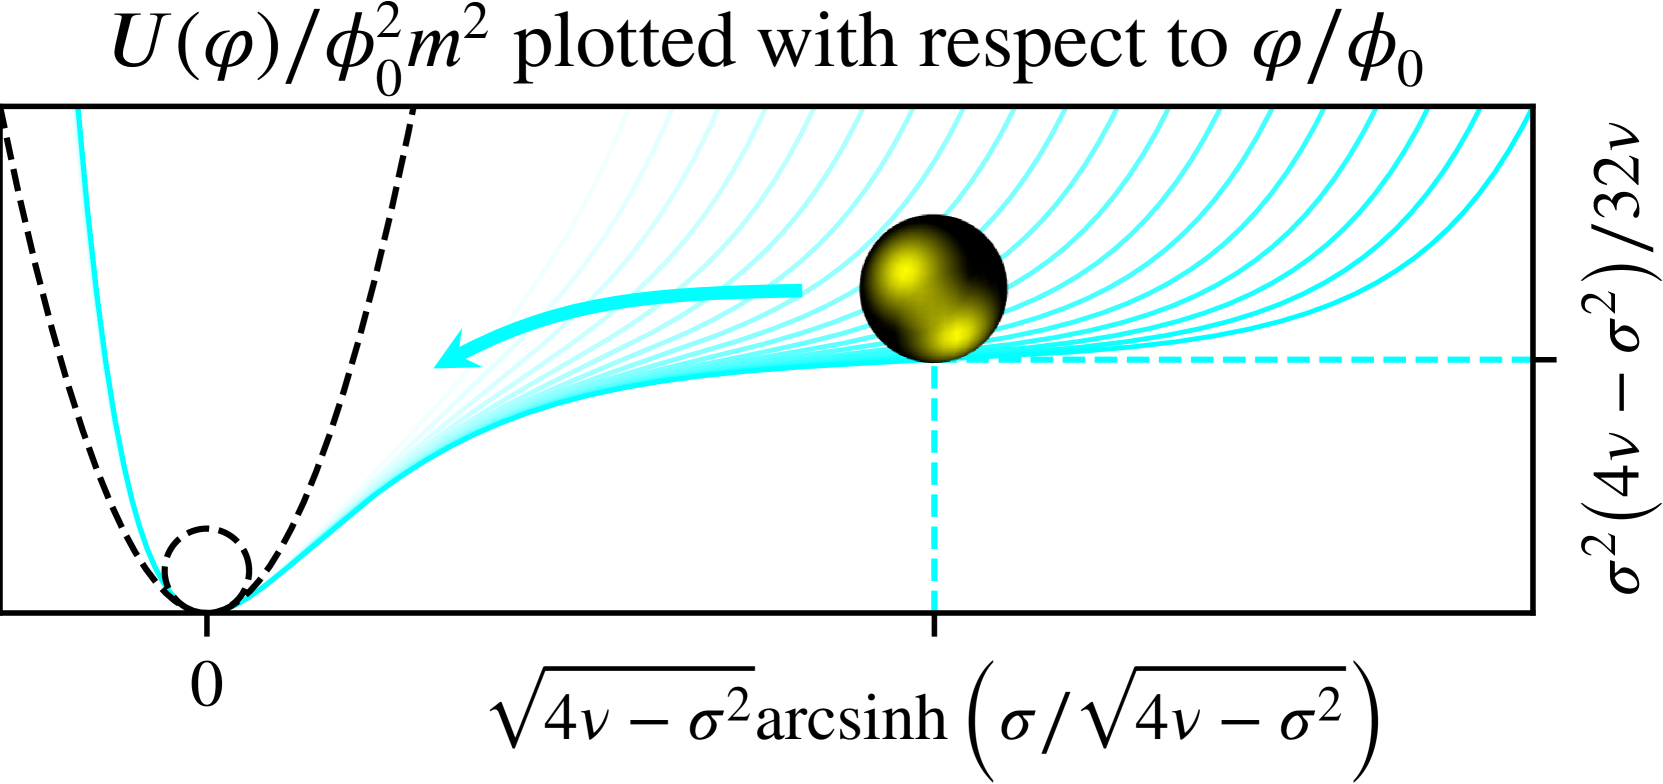
\includegraphics[width=0.5\textwidth]{Potential from Paper.png}
    \caption{Graph of the potential \cite{barker2024poincaregaugetheoryconformal}}
    \label{Potential from Paper}
\end{figure}


\section{Project Plan}

\subsection{Work Done}

In the first two weeks of the project, I reviewed the literature on the topic \cite{Mukhanov:2005sc}, \cite{baumann2012tasilecturesinflation}. This was to familiarize myself with the topics of cosmic inflation and the tools used to describe it. 

Upon getting a handle on the tools required, in week 3 and 4, I referred to the papers \cite{barker2024poincaregaugetheoryconformal} and \cite{Salvio_2022} to understand the derivation of the specific potential as described in section \ref{Section 3}. I also translated the equations to code and propagated the field to see how it would look.

To do this, the potential $U(\varphi)$ from section \ref{Section 3} equation \ref{26} was used in the equations \ref{21} to get a differential equation for the field $\varphi$. We also use the following relation to calculate the number of e-folds during inflation valid in the slow roll region,
\begin{equation}
    N(\varphi) = \int_{\phi_\text{end}}^{\phi} \frac{V}{V,_{\phi}} \mathrm{d}\varphi
\end{equation}
to fix the parameters [$\mu,\phi_0,\sigma,\nu,c$] = [1, 1.5, 11, 50, 0] such as to get the $N \approx 50.131$.

To plot the functions in a more self-evident manner, we use the relation $\mathrm{d}N = H \mathrm{d}t$ relating the number of efolds to the time, to rewrite the scalar field equation \ref{17} in terms of derivatives with respect to the number of efolds.

\begin{align}
    \ddot{\phi} + 3H\dot{\phi} + V,_\phi &= 0 
    \\
    H \frac{\mathrm{d}}{\mathrm{d}N} \left(H \frac{\mathrm{d}\phi}{\mathrm{d}N} \right) + 3 H^2 \frac{\mathrm{d}\phi}{\mathrm{d}N} + \frac{\mathrm{d}V}{\mathrm{d}\phi} &= 0    
\end{align}

Using the relations given by the Friedmann Equations \ref{2} and \ref{3}, we can simplify the final equation as:

\begin{equation}
    \frac{\mathrm{d}^2\phi}{\mathrm{d}N^2} + 3 \frac{\mathrm{d}\phi}{\mathrm{d}N} - \frac{1}{2} \left( \frac{\mathrm{d}\phi}{\mathrm{d}N} \right)^3 + \left[ 3 - \frac{1}{2} \left( \frac{\mathrm{d}\phi}{\mathrm{d}N} \right)^2 \right] \frac{\mathrm{d}\text{ln}V}{\mathrm{d}\phi}  = 0
\end{equation}

The resulting graphs obtained given the parameters can be seen below. 

This code is available in the \href{https://github.com/PrabhodaCS/Part-III-Inflation-Project}{GitHub repo} to check.

\newpage

\subsection{Goal of the Project and Timeline}

The end goal of this project is to focus on the further theoretical development of this model, such as the addition of extra so-called "compensator" fields, and the resulting implications for the potential. Unusual features present in the potential which could give rise to non-standard power spectra could also be explored. 
\subsection{Timeline}
\begin{itemize}
    \item \textbf{CHRISTMAS BREAK} :
    Moving forward, I will have to re-review the paper \cite{Salvio_2022} and \cite{Blas_2011}, to see the alternative formulation taken to get to a similar looking potential as in \ref{26}. This formulation assumes the connection coefficients of GR to be independent of the metric (Unlike in GR, where the connection coefficients are the Christoffel symbols, are derived by assuming metric compatibility). This means that there are two independent parameters with respect to which the variation of the action can be taken, leading to different dynamics. The immediate next steps for me is to translate the variables used there to the ones used in this approach and show it's equivalence. We will also explore the power spectra predicted by the theory next. Read all necessary literature to prepare myself for the Lent and Easter terms.

    \item \textbf{LENT TERM}
    
    \begin{itemize}
        \item Weeks 1-2 : Add different compensator fields and check how the potential changes. Graphing the different potentials and looking at it's results.
        \item Weeks 3-4 : Look into paper \cite{Salvio_2022} and try to implement a combination of scalar inflaton fields and spacetime with torsion (Connection is non metric compatable). This will change the shape of the potential and will have different power spectra.
        \item Weeks 5-6 : Finalize models worth exploring further. Calculate power spectra of these different models.
        \item Weeks 7- 8 : Compare the models with the Planck data and analyse the parameter space and valid values of couplings. Prepare the main results of the paper.
    \end{itemize}

    \item  \textbf{EASTER TERM} Prepare the results of the paper. Compare different models and analyze literature to find similar end results. Analyze how perturbations in the model could result in the current CMB anisotropy. Look into different ways model could be extended and matched with experimental data. Prepare for VIVA and final project submission.
\end{itemize}



\vspace{5\baselineskip}

\mbox{}\hfill
\signature{Dr. Will Barker}\hfill
\mbox{}

\printbibliography
\end{document}